\subsection{Influencia de las masas sobre estados de equilibrio de las comunidades receptoras}

A continuaci\'ion usamos la notaci\'on empleada en resultados siempre que sea posible.
\subsubsection{R-C}
Tenemos que al equilibrio $R$ y $C$ estan determinados por el siguiente par de expresiones
\begin{equation}
  \begin{aligned}
    R_{eq} &= \frac{q_{0,1} m_C^{\beta-h}}{\varepsilon_1 \alpha_{0,1} f_1(k_\RC)}\\
    C_{eq} &= \frac{r_0 m_C^{\beta -h}}{\alpha_{0,2} k_\RC^{1 - \beta}f_1(k_\RC)}(1 - \frac{R_{eq}}{\kappa_0 (k_\RC m_C)^{1-\beta}})
  \end{aligned}
\end{equation}

Las condiciones de existencia de equilibrio positivo son equivalentes a las condiciones para la invasi\'on de $C$ y se detallan en Resultados.\\
Dentro del espacio param\'etrico que posibilita la coexistencia tenemos asu vez que el efecto que causa cambios en $m_C(k_\CP m_P)$ es dependiente de la dimensi\'on del espacio de b\'usqueda: para espacios $3D$ tiene un impacto negativo sobre $R_{eq}$ y lo contrario ocurre en el caso $2D$. Su influencia sobre $C_{eq}$ es mas dif\'icil de diferenciar , en el caso $2D$ tenemos que el impacto es positivo, sin embargo en $3D$ depende del valor de $m_C$ ya que:
\begin{equation}
  \frac{\partial C_{eq}}{\partial m_C}  = d_0 ( (b-h) + (1 + 2h - 3 \beta )\frac{\chi_1}{\chi_0} m_C^{2\beta -h -1}) 
\end{equation}
Entonces la regi\'on de crecimiento y decrecimiento respecto a $m_C$ esta determinada por:
\begin{equation}
  \begin{cases}
    Crecimiento &  m_C^{1 + h - 2\beta} < \frac{q_{0,1}(1+2h -3 \beta)}{\chi_0(h - \beta)}\\
    Decrecimiento &  m_C^{1 + h - 2\beta} > \frac{q_{0,1}(1+2h -3 \beta)}{\chi_0(h - \beta)}
  \end{cases}
\end{equation}

\begin{figure}
  \centering
  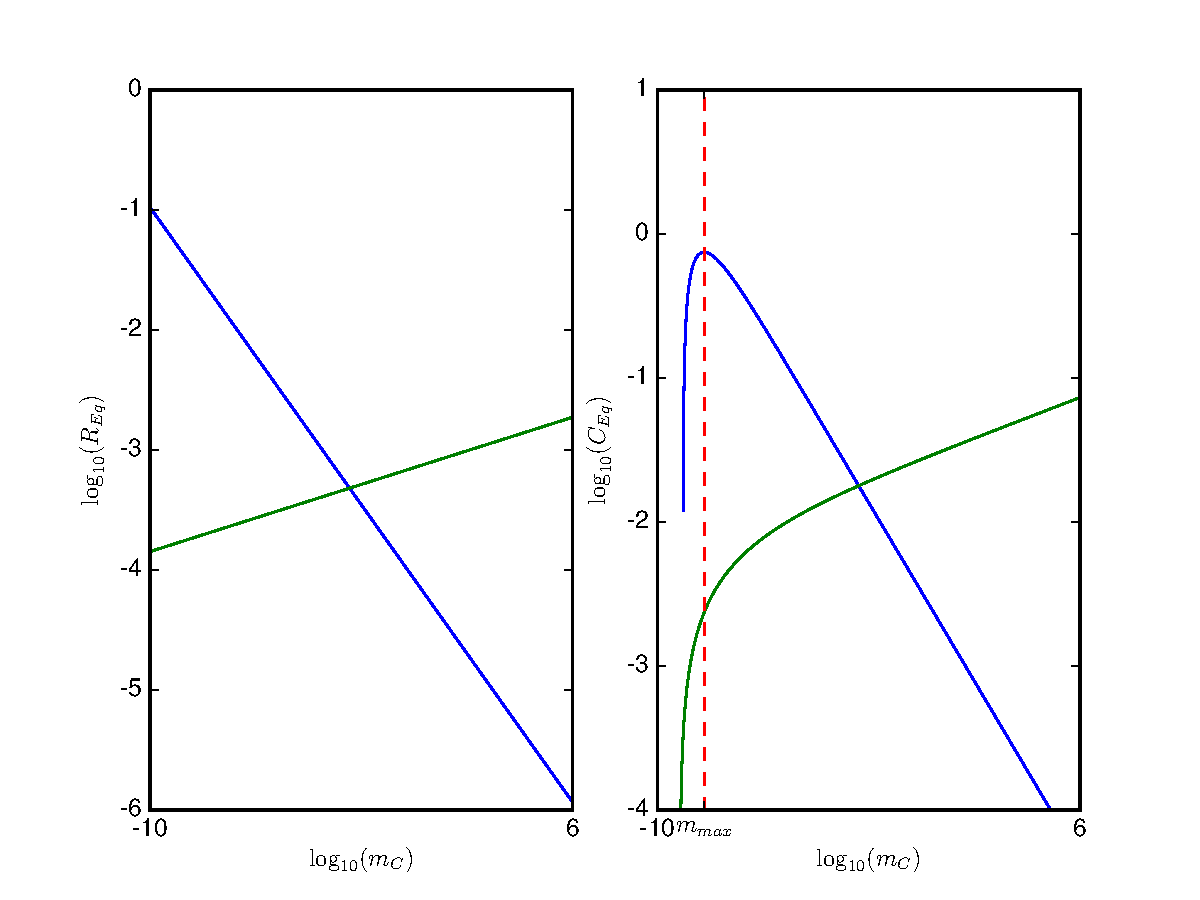
\includegraphics[width = 0.99\textwidth]{./Plots/RCeq.pdf}
  \caption[Equilibrio $R-C$vs$m_C$]{Equilibrios para el subsistema $R-C$ en funci\'on a $m_C$ para $k_\RC = 10^{-2}$, donde se observa las diferencias existentes entre espacios de b\'usqueda $2D$({\hwplotG}) y $3D$ ({\hwplotB}), en el panel de la derecha se representa a su vez el valor de $m_C$ para el cual $C_{eq}$ es m\'aximo.$b = 0.1$,$\kappa_0 = 0.1 , 30$  en espacios $2D$ y $3D$ respectivamente.}
  \label{fig:EqRCmC}
\end{figure}

La influencia de $k_\RC$(para un $m_C$ fijo)sobre los valores de equilibrio es an\'aloga a su influencia sobre la invasibilidad de $C$, dentro de la zona de coexistencia afecta negativamente a $R_{eq}$ en la zona de crecimiento de $f$ y positivamente en la zona de decrecimiento(si existiera), es decir se espera un valor m\'aximo de $R_{eq}$ para valores de $k_\RC$ cercanos a los l\'imites de coexistencia, la influencia sobre $C_{eq}$ al igual que en el caso anterior m\'as complicada teniendo:
\begin{equation}
  \frac{\partial C_{eq}}{\partial k_\RC}  = \frac{e_0 g'(k_\RC) }{g(k_\RC)^2} ( -1  + \frac{2e_1}{g(k_\RC)})
\end{equation}
Donde:
\begin{equation}
  \begin{aligned}
    e_0 &=  \frac{r_0 m_C^{\beta -h}}{\alpha_{0,2}} \\
    e_1 &=  \frac{q_{0,1} m_C^{2\beta-h-1}}{\varepsilon_1 \alpha_{0,1} \kappa_0}
  \end{aligned}
\end{equation}

Por tanto:
\begin{equation}
  \begin{cases}
    Crecimiento &  g'(k_\RC) ( \frac{2e_1}{g(k_\RC)} - 1) > 0 \\
    Decrecimiento &  g'(k_\RC) ( \frac{2e_1}{g(k_\RC)} - 1) < 0
    \end{cases}
\end{equation}

Dado que $g'(k_\RC)$ es positivo para $k_\RC$ peque\~nos y a su vez $g(k_\RC)$ disminuye , podemos esperar que para $k_\RC$ suficientemente peque\~nos $k_\RC$ afecte positivamente a $C_{eq}$ ,por otro lado dependiendo del valor de $\phi$ y la estrategia de forrajeo podemos tener un comportamiento cualitativo diferente para valores intermedios de $k_\RC$, en el caso m\'as simple $g'(k_\RC)$ siempre es positivo y por ende solo existir\'ia un punto de transici\'on entre zona de crecimiento y decrecimiento dado por la condici\'on $g(k_\RC) = 2e_1$ , sin embargo en el caso que $g(k_\RC)$ posea a su vez zonas de crecimiento y decrecimiento, observar\'iamos 3 transiciones $k_\RC^1 , k_\RC^2$ y$k_\RC^3$ , determinadas por $g(k_\RC^1) = 2e_1$ , $g'(k_\RC^2) =0$ y $g(k_\RC^3) = 2e_1$ , esto siempre que $k_\RC^1 < k_\RC ^2 < k_\RC^3$ ,es decir siempre que $g$ crezca los suficiente, en este caso observamos que $\kappa_0$ y $m_C$ favorecer\'ian la existencia de estos puntos debido a su influencia negativa sobre $e_1$.


\begin{figure}
  \centering
  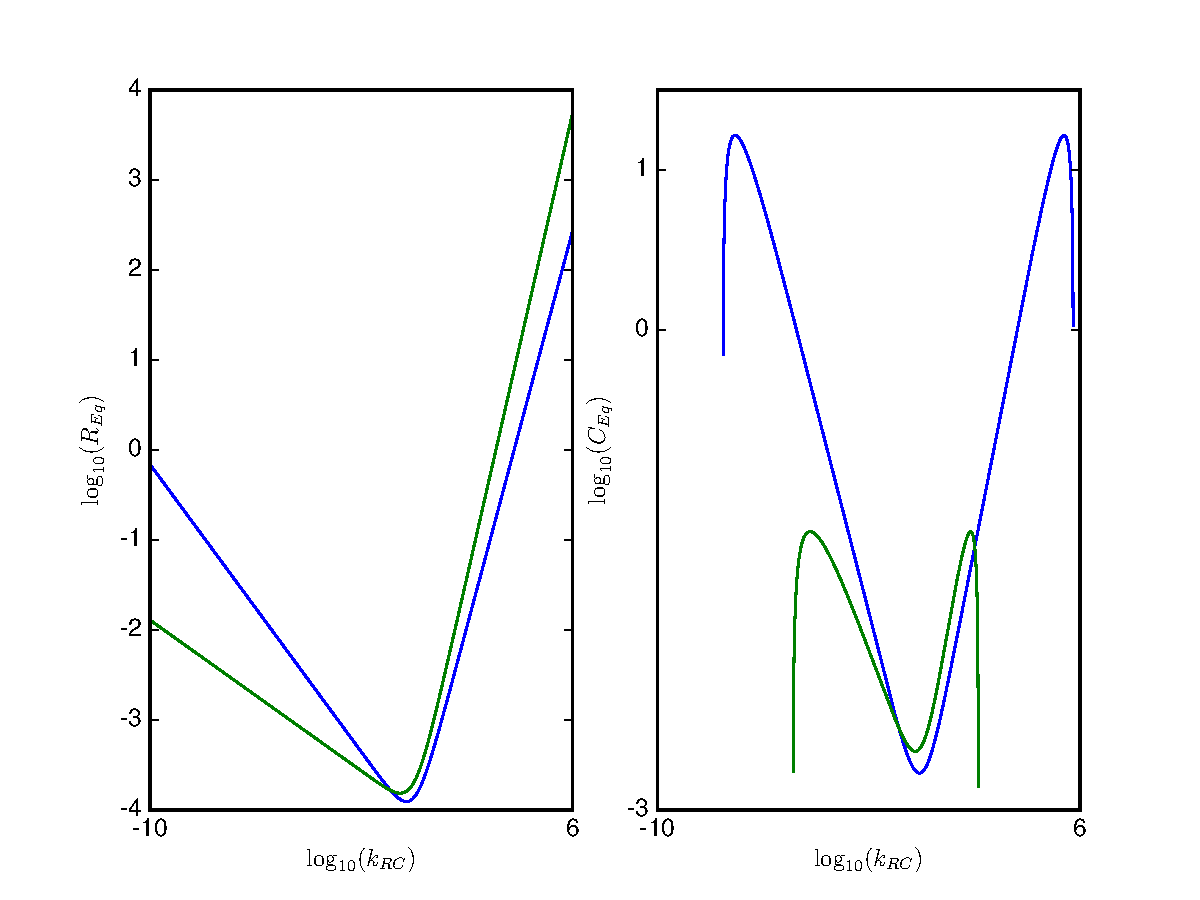
\includegraphics[width = 0.99\textwidth]{./Plots/RCeqKRC.pdf}
  \caption[Equilibrio $R-C$vs$k_\RC$]{Equilibrios para el subsistema $R-C$ en funci\'on a $k_\RC$ para $m_C = 10^{-3}$ , $b = 1.0 $,$\kappa_0 = 0.1 , 30$  en espacios $2D$ ({\hwplotG}) y $3D$ ({\hwplotB}) respectivamente. En el panel de la derecha se observan las tres transiciones entre zonas de crecimiento y decrecimiento, y en ambos casos la presencia de puntos m\'aximos cercanos a los l\'imites de coexistencia.}
  \label{fig:EqRCkRC}
\end{figure}

\subsubsection{R-P}
La descripci\'on es an\'aloga al caso anterior salvo que intercambiamos $m_C$ por $m_P$ y $k_\RC$ por $k_\RP$ en nuestro argumento.

\begin{equation}
  \begin{aligned}
    R_{eq} &= \frac{q_{0,2} m_P^{\beta-h}}{\varepsilon_2 \alpha_{0,2} f_2(k_\RP)}\\
    P_{eq} &= \frac{r_0 m_P^{\beta -h}}{\alpha_{0,2} k_\RP^{1 - \beta}f_2(k_\RP)}(1 - \frac{R_{eq}}{\kappa_0 (k_\RP  m_P)^{1-\beta}})
  \end{aligned}
\end{equation}







